% !TEX root = pfe-book2.tex
%!TEX TS-program = pdflatex
%!TEX encoding = UTF-8 Unicode


\cleardoublepage
%\mainmatter
\chapter{Transformations of Molecules}
\label{ch-07}

\section{Chemical Reactions}

Physics is the foundation of all natural sciences. It is therefore absolutely impossible to separate physics from chemistry, geology, meteorology, biology and all the other branches of science. The basic laws of nature come under the topic of physics. It is no mere chance then that books have been written on geological physics, biological phys­ics, chemical physics, construction physics, etc. Hence, we find it appropriate to devote a section to chemical reactions in this book which deals with the basic laws of nature.

Strictly speaking, chemistry begins where a molecule is broken down into its component parts, or when a single molecule is formed of two others, or when two colliding molecules are converted into two other molecules. If we find that from the beginning to the end of a phenome­non a change has occurred in the chemical composition of the bodies involved, then a reaction has taken place.

Chemical reactions can occur ``on their own'', i.e. due to the motions of the molecules at the given temperature. Hence, we often say that a substance decomposes. This means that the internal vibrations of the atoms in the molecules rupture the bonds between the atoms and the molecule ``falls apart''.

A chemical reaction is most often the result of encoun­ters between molecules. A metal rusts. This is a chemical reaction; an atom of the metal encounters a molecule of water, and an oxide is formed. A pinch of citric acid and a spoon of soda are mixed into a glass of water. Bubbles of gas begin to evolve vigorously. The encounter of these two kinds of molecules has resulted in the formation of new substances, including carbon dioxide whose bubbles rise to the surface and burst.

Hence, spontaneous disintegration of molecules and collision of molecules are two causes of chemical reactions. But chemical reactions may be due to other causes as well. You are vexed when you examine the suit of clothes that you took along on your vacation trip to the south. The cloth has faded and lost its true colour. Owing to intense action of the Sun’s rays, a chemical transforma­tion has occurred in the dye.

Reactions induced by light are said to be photochemical. Investigations in this field must be especially carefully conducted to distinguish heat-induced reactions, due to heat generated by light (which increases the kinetic ener­gy of motion of molecules so that their collisions are more frequent and more violent), from reactions directly induced by light. In the latter, particles of light -- pho­tons -- ``rupture'' the chemical bonds.

The action of light is responsible for the chain of chem­ical reactions that take place in green plants, and which is called photosynthesis. The photochemical transforma­tion occurring in living plants realizes the great carbon cycle without which life would be impossible.

Chemical bonds may be ruptured in various chemical reactions by other energetic particles as well, such as electrons, protons, etc.

Chemical reactions may proceed either with the absorp­tion of heat or with its evolution. What does this signify at the molecular level? If two slow molecules meet and form two fast ones, then heat has been generated because we know that an increase in temperature is equivalent to an acceleration of the molecules. Such reactions include combustion and explosion, which we are to discuss in the next section.

Next we shall consider the reaction rate from the molec­ular point of view, i.e. at the molecular level. Just about everyone knows that some reactions are completed faster than you can blink an eye (say, explosions), while others take years. Assume that we are again concerned with reactions in which two molecules collide and form two other molecules. The following assumption is evidently true. Of significance, in the first place, is collision energy of an amount sufficient to break up the molecules and to rearrange them. Also important, in the second place, is whether the reaction proceeds regardless of the angle at which the molecules meet in collision or whether they must meet at certain angles.

The minimum energy required to implement a reac­tion is called the activation energy. It plays the chief role in the course of the reaction, but we must give its due to a second factor as well -- the percentage of ``lucky'' colli­sions of particles having a given energy.
\begin{figure}[!ht]
\centering
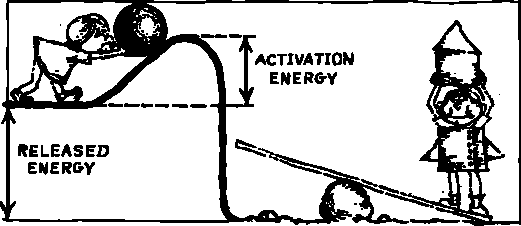
\includegraphics[width=\textwidth]{figures/fig-07-01.pdf}
\caption{A schematic of heat producing chemical reaction in terms of energy.}
\label{fig-7.1}
\end{figure}
A heat-producing chemical reaction can be modelled as shown in \figr{fig-7.1}. The ball rolls uphill, over the barrier and drops down. Since the initial energy level is higher than the final one, more energy is produced than has been expended.

This mechanical model visually illustrates the critical dependence of the reaction rate on the temperature. If the temperature is low, the ``speed'' of the ball is insuffi­cient to surmount the barrier. As the temperature increas­es, the number of balls leaping over the barrier increases faster and faster. The rate of chemical reactions depends to an exceptionally great extent on the temperature. As a rule, a temperature increase of 10 degrees speeds up a reaction from two- to four-fold. If the reaction rate is, say, tripled when we raise the temperature 10 degrees, then a temperature increase of 100 degrees leads to a rate increase of $\num{3d10}\approx  \num{60 000}$ times, 200 degrees to $\num{3d20} \approx  \num{4d9}$, and 500 degrees to \num{3d50}, i.e. approximately \num{d24} times. No wonder then that a reaction proceeding at a normal rate at \SI{500}{\celsius} does not take place at all at room temperature.

\section{Combustion and Explosion}

For combustion to begin, it is necessary, as is well known, to bring a burning match to an inflammable object. But neither does a match light up by itself; it must be struck against a match-box. Therefore, in order that a chemical reaction start, a preliminary heating is necessary. The ignition creates the required temperature for the reaction at the initial moment. A high temperature is further maintained by the heat which is liberated in the course of the reaction.

The initial local heating should be sufficient for the heat liberated by the reaction to exceed that transferred to the cold surrounding medium. Therefore, each reac­tion has its own, as one says, \emph{ignition point}. 
Combustion only begins if the initial temperature is higher than the ignition point. For example, the ignition point of wood is \SI{610}{\celsius}, of benzine about \SI{200}{\celsius}, of white phosphorus \SI{50}{\celsius}.

The combustion of wood, coal or oil is a chemical reac­tion uniting the substance with the oxygen of the air. Therefore, such a reaction proceeds at the surface: until the outside layer burns up, the next layer cannot participate in the combustion. This is what explains the rela­tive slowness of such combustion. It is not difficult to convince oneself in practice of the validity of what we have said. If fuel is broken up into small pieces, the rate of combustion may be considerably increased. This is why the crushing of coal is carried out in furnaces.

Fuel fed to the cylinder of an internal-combustion en­gine is broken down and mixed with air in exactly the same way. More complex substances than coal are used for engine fuel, for instance, gasoline. A molecule of such a substance is shown in \figr{fig-7.2} at the left. It consists of 8 carbon atoms and 18 hydrogen atoms bonded together as shown. As it burns, this molecule is subject to colli­sions from oxygen molecules. These collisions break up the gasoline molecules. The forces that join one or two carbon atoms to a hydrogen atom in a molecule, and those that join two oxygen atoms to make up an oxygen mole­cule, cannot withstand the stronger ``affinity'', as chemists say, between oxygen atoms, on the one hand, and carbon and hydrogen atoms, on the other. Consequently, the old bonds between the atoms in a molecule are ruptured and the atoms are rearranged into new molecules. As is indi­cated in \figr{fig-7.2} at the right, the new molecules --com­bustion products -- consist of carbon dioxide and water. Water is produced in the form of steam.
\begin{figure}[!ht]
\centering
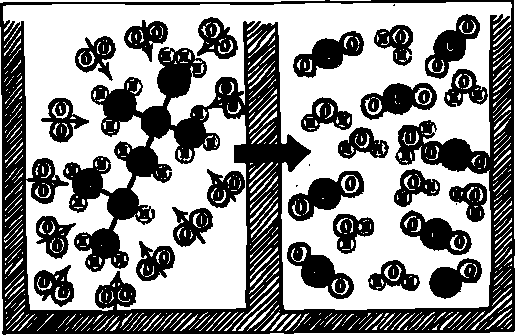
\includegraphics[width=\textwidth]{figures/fig-07-02.pdf}
\caption{A combustion reaction.}
\label{fig-7.2}
\end{figure}

The situation is entirely different in the case where the atmosphere is not needed, where everything that is necessary for the reaction is contained within the sub­ stance. An example of such a substance is a mixture of hydrogen and oxygen (it is called a detonating gas). The reaction occurs not at the surface but within the substance. Unlike the case of combustion, all the energy forming in the course of the reaction is liberated almost instanta­neously, as a result of which the pressure rises sharply and an explosion takes place. A detonating gas doesn’t burn -- it explodes.

Thus, an explosive should contain within it the atoms or molecules needed for a reaction. It is evident that we can prepare explosive gas mixtures. There also exist solid explosives. They are explosive precisely because in their compositions all atoms occur which are necessary for chemical reactions giving off heat and light.
\begin{figure}[!ht]
\centering
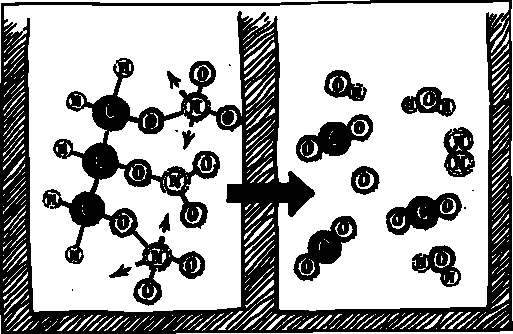
\includegraphics[width=\textwidth]{figures/fig-07-03.pdf}
\caption{An example of explosive reaction using nitroglycerine.}
\label{fig-7.3}
\end{figure}

The chemical reaction taking place during an explosion is a decomposition reaction of the splitting up of mole­cules into parts. An example of an explosive reaction is shown in \figr{fig-7.3} -- the splitting up of a nitroglycerine molecule into its parts. As is evident from the right-hand part of the diagram, molecules of carbon dioxide, water and nitrogen are formed out of the original molecule. We find the ordinary combustion products among the end products, but combustion has occurred without the par­ticipation of oxygen molecules from the air; all atoms necessary for the combustion are contained within the nitroglycerine molecule.

How is an explosion propagated through an explosive, for example, a detonating gas? When we set fire to an explosive, a local heating arises. A reaction occurs in the heated region. But heat is liberated in the course of the reaction, and passes into the adjacent layers of the mixture by means of heat transfer. This heat is sufficient for the reaction to take place in the neighbouring layer, too. New amounts of the heat being liberated enter the next layers of the detonating gas, and so with the rate of heat transfer the reaction spreads throughout the entire substance. The rate of such a transfer is of the order of 20-30 \si{\meter\per\second}. This is, of course, very rapid. A metre-long tube of gas explodes within one-twentieth of a second, i.e. almost instantaneously, while the rate of the combus­tion of wood or pieces of coal that takes place at the sur­face, and not within the volume, is measured in centime­tres per minute, i.e. is several thousand times less.

Nevertheless, such an explosion may also be called slow, since a different kind of explosion, hundreds of times faster than the one described, is possible.

A shock wave gives rise to a fast explosion. If the pres­sure rises sharply in some layer of a substance, a shock wave will begin propagating from this place. A shock wave leads to a considerable jump in temperature which is transmitted from layer to layer. The rise in tempera­ture gives an impetus to an explosive reaction, and the explosion leads to a rise in pressure and maintains the shock wave, whose intensity would otherwise fall off rapidly with its propagation. Therefore, a shock wave gives rise to an explosion, while the explosion in turn maintains the shock wave. The type of explosion described by us is called a detonation. Since a detonation is propagated through a substance with the speed of a shock wave (of the order of \SI{1}{\kilo\meter\per\second}), it is actually hundreds of times faster than a ``slow'' explosion.\label{explosion}

But which substances explode ``slowly'' and which explode ``rapidly''? The question should not be posed in this fashion: one and the same substance can explode “slowly” and also detonate under different conditions, while a “slow” explosion turns into a detonation in cer­tain cases.

Some substances, for example, nitrogen iodide, explode on contact with a straw, on being slightly heated or as a result of a flash of light. An explosive substance like trotyl does not explode when it is dropped or even shot out of a rifle. A powerful shock wave is required in order to explode it.


There exist substances even less sensitive to external influences. The fertilizing mixture of ammonium nitrate and ammonium sulfate had not been considered to be explosive until a tragic accident occurred in 1921 at a chemical factory in Oppau, Germany. An explosive meth­od was used there for pulverizing mixtures which had become caked. As a result, a warehouse and the entire factory were blown up. The engineers at the factory could not be blamed for the catastrophe: approximately twen­ty thousand blasts had proceeded normally, and only once had the conditions favourable for detonation been creat­ed.

Substances which explode only when subjected to a shock wave but exist in a stable state and are not even afraid of fire under ordinary conditions are quite conve­nient for explosion technology. Such substances can be manufactured and stored in large amounts. However, in order to bring these inert explosives into action, initia­tors of the explosion are needed. Such initiating explo­sives are absolutely necessary as sources of shock waves.

Mercury fulminate can serve as an example of initia­tors. If a grain of it is placed on a sheet of tin and lighted, an explosion takes place, making a hole in the tin. An explosion of such a substance under any conditions is a detonation.

If a bit of mercury fulminate is placed on the charge of a secondary explosive and lighted, the explosion of the initiator creates a shock wave which is enough to deto­nate the secondary explosive. Explosions are produced in practice with the aid of a detonating capsule (1-2 \si{\gram} of an initiator). The capsule can be ignited at a distance, for example, with the aid of a long cord (Bickford fuse); the shock wave coming from the capsule will blow up the secondary explosive.

In a number of cases arising in technology, we must contend with detonations. ``Slow explosions'' of a mixture of gasoline and air occur in the motor of a car under ordi­nary conditions. However, sometimes a detonation also arises. Shock waves in a motor are absolutely unaccept­able as a systematic phenomenon, since they will soon put the walls of the cylinders of the motor out of commis­sion.

In order to cope with detonations in engines, it is nec­essary to either use a special gasoline with a high oc­tane number or else mix the gasoline with special substances, antiknocks, which do not let a shock wave de­velop. One of the most widespread antiknocks is tetra­ ethyl lead (TEL). This substance is highly toxic, and so drivers are warned of the need to be careful when using such gasoline.\footnote{As of 2021, the use of leaded petrol has been ended globally. -- Damitr}

Cannons must be constructed so as to avoid detona­tions. Shock waves should not be formed inside the barrel when the gun is being fired, otherwise, the gun will be put out of commission.

\section[Engines Operated by Transformations of Molecules]{Engines Operated by \\Transformations of Molecules}
People living in the 20th century use a great variety of engines and motors to help them do their work and to increase their power about ten-fold.

In the simplest case, it may prove expedient to convert mechanical energy into another kind of mechanical ener­gy. For instance, we may have the wind or a stream of water rotate the vanes of a windmill or the water wheel of a mill.

In a hydroelectric power station, the process of converting the energy of a stream of water into rotary motion of the turbine runner is an intermediate one. The tur­bine drives an electrical machine, called a generator, which produces electricity. Such conversion of energy will be discussed further on.

Steam engines have become things of the past. A steam locomotive is fast becoming a rarity to be exhibited in museums. This has occurred because the efficiency of a heat engine is much too low.

This does not imply that steam turbines have become obsolete. But there as well the conversion of the energy of expanding steam into mechanical motion of the rotor is only an intermediate stage. The final stage is the production of electrical power.

As to aircraft and automobiles, there is obviously no point in powering them with a steam boiler or steam tur­bine. The total weight of the engine and heating device proves too great when calculated on a kilograms per horse power basis.

We can, however, eliminate the separate heating plant. In a gas turbine, the immediate working fluid consists of the incandescent combustion products of a high-ener­gy fuel. In such engines, we use chemical reactions, i.e. transformations of molecules, to produce mechanical energy. This is what determines both the significant ad­ vantages of gas turbines over the steam-powered type, and the great design and manufacturing difficulties that have to be overcome to ensure their reliable perfor­mance.

The advantages are obvious: the combustion chamber, where the fuel is burned, has a small size and can be placed under the casing of the turbine. The components of combustion consisting, for example, of atomized kero­sene and oxygen have a temperature unattainable for steam. The heat flow formed in the combustion chamber of a gas turbine is very intense, which makes it possible to obtain a high efficiency.

But these advantages turn into shortcomings. The steel blades of the turbine function in streams of gas having a temperature up to \SI{1200}{\celsius} and inevitably saturated with microscopic ash particles. It is easy to imagine what great demands have to be made of the materials out of which gas turbines are manufactured.

During an attempt to construct a gas turbine with a power of about 200 hp for an automobile, it became nec­essary to deal with quite a peculiar difficulty: the tur­bine was of such small dimensions that the usual engineering solutions and the customary materials simply could not be used. However, the technological difficul­ties are already being overcome. The first automobiles powered by gas turbines have been designed and built, but it is difficult to foresee their future.

It turned out easier to utilize the gas turbine in rail­ way transport. Locomotives with gas turbines, gas-tur­bine locomotives, have already received universal rec­ognition.

But entirely different engines in which the gas turbine is a subordinate although necessary component part paved the way for the widespread use of the gas turbine. We are speaking of the turbojet engine, the basic type of
engine at the present time in jet aviation.

The principle on which the jet engine is based is simple.

A gas mixture is burned in a durable combustion cham­ber; the combustion products, having an extraordinarily great speed (\SI{3000}{\meter\per\second}, when hydrogen is burned in oxy­gen, somewhat less for other types of fuel), are thrust through a smoothly expanding nozzle in the direction op­posite to that of motion. Even relatively small amounts of combustion products will carry a large momentum away from the engine.
With the creation of jet engines, people received the realistic opportunity of carrying out interplanetary flights.

Liquid propellant rocket engines have become very widespread. Definite portions of a fuel (for example, ethyl alcohol) and an oxidizer (usually liquid oxygen) are injected into the combustion chamber of such an engine. The mixture burns, creating traction. In high-altitude rockets, such as the $V$-2, the traction is of the order of 15 tonf. The figures are sufficiently eloquent: 8.5 tons of fuel and oxidizer which take 1.5 minutes to burn up are poured into the rocket. The use of liquid pro­pellant rocket engines is only expedient for flights at great heights or beyond the Earth’s atmosphere. It makes no sense to pour large amounts of a special oxidizer into an aircraft destined for flights in the lower layers of the atmosphere (up to \SI{20}{\kilo\meter}), where there is enough oxygen. But then the problem arises of forcing huge amounts of air necessary for intensive burning into the combustion chamber. This problem is solved in a natural fashion: part of the energy of the gas stream created in the com­bustion chamber is taken away to rotate the powerful compressor forcing air into the chamber.
\begin{figure}[!ht]
\centering
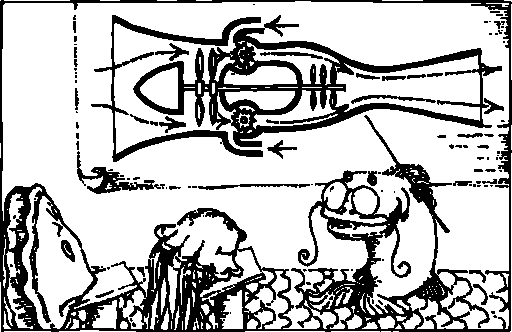
\includegraphics[width=\textwidth]{figures/fig-07-04.pdf}
\caption{A schematic of a turbojet engine.}
\label{fig-7.4}
\end{figure}
We have already said what engine can do work at the expense of the energy of a stream of incandescent gases; of course, this is the gas turbine. The whole system is called a turbojet engine (\figr{fig-7.4}). A turbojet engine has no competitor for flights with speeds from 800 to \SI{1200}{\kilo\meter\per\hour}.

For long-distance flights with speeds of 600-\SI{800}{\kilo\meter\per\hour} an ordinary aircraft propeller is added to the shaft of a turbojet engine. This is a turboprop engine.

At flying speeds of about  \SI{2000}{\kilo\meter\per\hour} or more, the air pressure developed by the aircraft is so great that the need for a compressor no longer arises. It is then only nat­ural that neither is a gas turbine needed. The engine is converted into a pipe of variable cross-section, in which fuel is burned at a very definite place. This is a ramjet engine. It is clear that a ramjet engine cannot lift an aircraft off the ground: it becomes capable of function­ing only at very high flying speeds.

Jet engines are completely inexpedient for flights at small speeds owing to the large expenditures of fuel. For motion on land, on water or in air with speeds from 0 to  \SI{500}{\kilo\meter\per\hour}, people are reliably served by gasoline or diesel internal-combustion piston engines. As indicated by the name, the main part of such an engine is the cyl­inder inside which the piston can move. The back-and-forth motion of the piston is transformed into a rotary motion of the shaft with the aid of the connecting rod and crank system (\figr{fig-7.5}).
\begin{figure}[!ht]
\centering
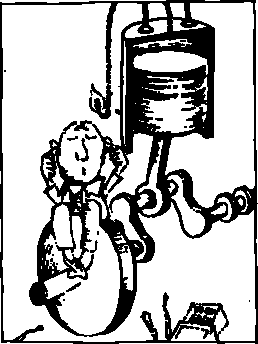
\includegraphics[width=0.4\textwidth]{figures/fig-07-05.pdf}
\caption{An internal combustion engone.}
\label{fig-7.5}
\end{figure}
The motion of the piston is transmitted through the con­necting rod to the crank, which is part of the crankshaft. The motion of the crank sets the shaft into rotation. Con­versely, if the crankshaft is turned, this will move the connecting rods and a displacement of the pistons inside the cylinders will set in.

The cylinder of a gasoline engine is equipped with two valves, one of which is meant for the inlet of the fuel mix­ture, and the other for the exhaust of waste gases. In order to start the engine, we must turn it over, using the energy of some outside source. Assume that at a cer­tain moment the piston is moving down and the inlet valve is open. A mixture of atomized gasoline and air is sucked into the cylinder. The inlet valve is connected to the shaft of the engine in such a way that it closes at the moment when the piston reaches its lowest position. As the shaft continues to turn, the piston starts coming up. The automatic drive of the valves keeps then closed dur­ing this stroke, and the fuel mixture is therefore compres­sed. When the piston reaches its highest position, the compressed mixture is ignited by an electric spark, which jumps between the electrodes of the spark plug. The mixture ignites and the expanding combustion products act, pushing the piston down. The engine shaft receives a powerful thrust, and the flywheel on the shaft stores considerable kinetic energy. All of the next three preliminary strokes proceed at the expense of this energy: first the exhaust, when the exhaust valve is open and the piston is moving up, driving the exhaust out of the cylinder, next the intake and compression that we already know about, then a new ignition. The engine is started. 

Gasoline engines have powers from fractions of a horse­ power to 4000~hp, an efficiency of up to 40\% and weigh up to 300~gf per horsepower. Their widespread utiliza­tion in automobiles and aircrafts is explained by such a good showing.

How might we increase the efficiency of a gasoline engine? The major means is by raising the degree of com­pression.

If the fuel mixture is more highly compressed before ignition, it will have a higher temperature. And why is it of advantage to raise its temperature? The point is that we can rigorously prove that the maximum attainable efficiency equals $1-T/T_{0}$, where $T$ is the temperature of the working body, and $T_{0}$ is the ambient temperature. This proof is tedious and uninteresting, and we omit it. In numerous instances we have asked our readers to just take our word for various statements. Since the ambient temperature, i.e. the temperature of the surrounding me­dium, is something we cannot do much about, we make every effort to raise the temperature of the working body as high as is feasible. But -- there, unfortunately, is a but -- a highly compressed fuel mixture detonates (see page~\pageref{explosion}). Then the working stroke acquires the features of a heavy explosion which may damage the engine.

One has to take special measures to decrease the deto­nation properties of the gasoline, and this would greatly raise the cost of a fuel that is already quite expen­sive.

The problems of raising the temperature during the working stroke, of eliminating detonation and reducing the cost of the fuel have been successfully solved in the diesel engine.

A diesel engine resembles a gasoline engine to a great extent in its construction, but is designed for products of oil distillation which are cheaper than and inferior in quality to gasoline.

The cycle begins with the admission of pure air into the cylinder. The air is then compressed by the piston to approximately \SI{20}{\atmos}. It would be very difficult to achieve such a high compression by turning over the engine by hand. Therefore, diesel engines are started with a special starting motor, usually a gasoline one, or by compressed air.

When highly compressed, the temperature of the air in a cylinder rises so much that it becomes sufficient for the fuel mixture to ignite. But how can it be admitted into the cylinder, where a high pressure has been attained? An inlet valve would not be suitable here. It is replaced by a sprayer which forces the fuel into the cylinder through a tiny opening. It ignites as it enters, eliminating the danger of a detonation considerable for a gasoline engine.
Eliminating the danger of a detonation permits us to construct slow diesels with many thousands of horsepow­ers. Naturally, they acquire quite considerable dimen­sions, but remain more compact than an aggregate consisting of a steam boiler and a turbine.

A ship in which there are direct-current generator and motor between a diesel engine and a blade is called a diesel-electric motor ship.
Diesel locomotives, now being widely introduced on railroads, are built along the same lines; they may in a sense be called diesel-electric locomotives.

Internal-combustion piston engines, considered last by us, have borrowed their basic constructive elements -- the cylinder, the piston, the connecting rod and crank mechanism which helps obtain rotary motion -- from the steam engine, now gradually leaving the scene. The steam engine could have been called an ``external-combustion piston engine'' It is precisely this combination of the unwieldy steam boiler with the no less unwieldy system of transforming translatory motion into rotary one that deprives the steam engine of the possibility of successfully competing with more modern engines.

Modern steam engines have an efficiency of about 10\%. The locomotives which have been taken out of production released up to 95\% of the fuel they burned through the smoke-stack to no advantage.

This ``record-breaking'' low efficiency is explained by the inevitable deterioration in the properties of a steam boiler designed for installation on locomotive as com­pared to a stationary steam boiler.

But why were steam engines employed so widely in transportation for such a long time? Besides adherence to customary solutions, the circumstance that a steam en­gine has a very good tractive characteristic also played a role: the greater the force with which the load resists a displacement of the piston, the greater the force exerted on it by the steam, i.e. the torque developed by a steam engine grows under difficult conditions, which is important in transportation. But, of course, the fact that the steam engine does not need a complicated system of variable transmission to the driving axles cannot in the least compensate for its basic defect, a low efficiency. This is what explains the supplanting of the steam engine by other engines.